% !TEX program = xelatex
\documentclass[a4paper,14pt,oneside,openany]{memoir}

%%% Задаем поля, отступы и межстрочный интервал %%%
\usepackage{amsmath}
\usepackage[left=30mm, right=15mm, top=20mm, bottom=20mm]{geometry} % Пакет geometry с аргументами для определения полей
\pagestyle{plain} % Убираем стандарные для данного класса верхние колонтитулы с заголовком текущей главы, оставляем только номер страницы снизу по центру
\parindent=1.25cm % Абзацный отступ 1.25 см, приблизительно равно пяти знакам, как по ГОСТ
\usepackage{indentfirst} % Добавляем отступ к первому абзацу
%\linespread{1.3} % Межстрочный интервал (наиболее близко к вордовскому полуторному) - тут вместо этого используется команда OnehalfSpacing*

%%% Задаем языковые параметры и шрифт %%%

\usepackage[english, russian]{babel}                % Настройки для русского языка как основного в тексте
\babelfont{rm}{Times New Roman}                     % TMR в качестве базового roman-щрифта

%%% Задаем стиль заголовков и подзаголовков в тексте %%%

\setsecnumdepth{subsection} % Номера разделов считать до третьего уровня включительно, т.е. нумеруются только главы, секции, подсекции
\renewcommand*{\chapterheadstart}{} % Переопределяем команду, задающую отступ над заголовком, чтобы отступа не было
\renewcommand*{\printchaptername}{} % Переопределяем команду, печатающую слово "Глава", чтобы оно не печалось
%\renewcommand*{\printchapternum}{} % То же самое для номера главы - тут не надо, номер главы оставляем
\renewcommand*{\chapnumfont}{\normalfont\bfseries} % Меняем стиль шрифта для номера главы: нормальный размер, полужирный
\renewcommand*{\afterchapternum}{\hspace{1em}} % Меняем разделитель между номером главы и названием
\renewcommand*{\printchaptertitle}{\normalfont\bfseries\centering\MakeUppercase} % Меняем стиль написания для заголовка главы: нормальный размер, полужирный, центрированный, заглавными буквами
\setbeforesecskip{20pt} % Задаем отступ перед заголовком секции
\setaftersecskip{20pt} % Ставим такой же отступ после заголовка секции
\setsecheadstyle{\raggedright\normalfont\bfseries} % Меняем стиль написания для заголовка секции: выравнивание по правому краю без переносов, нормальный размер, полужирный
\setbeforesubsecskip{20pt} % Задаем отступ перед заголовком подсекции
\setaftersubsecskip{20pt} % Ставим такой же отступ после заголовка подсекции
\setsubsecheadstyle{\raggedright\normalfont\bfseries}  % Меняем стиль написания для заголовка подсекции: выравнивание по правому краю без переносов, нормальный размер, полужирный

%%% Задаем параметры оглавления %%%

\addto\captionsrussian{\renewcommand\contentsname{Содержание}} % Меняем слово "Оглавление" на "Содержание"
\setrmarg{2.55em plus1fil} % Запрещаем переносы слов в оглавлении
%\setlength{\cftbeforechapterskip}{0pt} % Эта команда убирает интервал между заголовками глав - тут не надо, так красивее смотрится
\renewcommand{\aftertoctitle}{\afterchaptertitle \vspace{-\cftbeforechapterskip}} % Делаем отступ между словом "Содержание" и первой строкой таким же, как у заголовков глав
%\renewcommand*{\chapternumberline}[1]{} % Делаем так, чтобы номер главы не печатался - тут не надо
\renewcommand*{\cftchapternumwidth}{1.5em} % Ставим подходящий по размеру разделитель между номером главы и самим заголовком
\renewcommand*{\cftchapterfont}{\normalfont\MakeUppercase} % Названия глав обычным шрифтом заглавными буквами
\renewcommand*{\cftchapterpagefont}{\normalfont} % Номера страниц обычным шрифтом
\renewcommand*{\cftchapterdotsep}{\cftdotsep} % Делаем точки до номера страницы после названий глав
\renewcommand*{\cftdotsep}{1} % Задаем расстояние между точками
\renewcommand*{\cftchapterleader}{\cftdotfill{\cftchapterdotsep}} % Делаем точки стандартной формы (по умолчанию они "жирные")
\maxtocdepth{subsection} % В оглавление попадают только разделы первыхтрех уровней: главы, секции и подсекции

%%% Выравнивание и переносы %%%

%% http://tex.stackexchange.com/questions/241343/what-is-the-meaning-of-fussy-sloppy-emergencystretch-tolerance-hbadness
%% http://www.latex-community.org/forum/viewtopic.php?p=70342#p70342
\tolerance 1414
\hbadness 1414
\emergencystretch 1.5em                             % В случае проблем регулировать в первую очередь
\hfuzz 0.3pt
\vfuzz \hfuzz
%\dbottom
%\sloppy                                            % Избавляемся от переполнений
\clubpenalty=10000                                  % Запрещаем разрыв страницы после первой строки абзаца
\widowpenalty=10000                                 % Запрещаем разрыв страницы после последней строки абзаца
\brokenpenalty=4991                                 % Ограничение на разрыв страницы, если строка заканчивается переносом

%%% Объясняем компилятору, какие буквы русского алфавита можно использовать в перечислениях (подрисунках и нумерованных списках) %%%
%%% По ГОСТ нельзя использовать буквы ё, з, й, о, ч, ь, ы, ъ %%%
%%% Здесь также переопределены заглавные буквы, хотя в принципе они в документе не используются %%%

\makeatletter
    \def\russian@Alph#1{\ifcase#1\or
       А\or Б\or В\or Г\or Д\or Е\or Ж\or
       И\or К\or Л\or М\or Н\or
       П\or Р\or С\or Т\or У\or Ф\or Х\or
       Ц\or Ш\or Щ\or Э\or Ю\or Я\else\xpg@ill@value{#1}{russian@Alph}\fi}
    \def\russian@alph#1{\ifcase#1\or
       а\or б\or в\or г\or д\or е\or ж\or
       и\or к\or л\or м\or н\or
       п\or р\or с\or т\or у\or ф\or х\or
       ц\or ш\or щ\or э\or ю\or я\else\xpg@ill@value{#1}{russian@alph}\fi}
\makeatother

%%% Задаем параметры оформления рисунков и таблиц %%%

\usepackage{graphicx, caption, subcaption} % Подгружаем пакеты для работы с графикой и настройки подписей
\graphicspath{{images/}} % Определяем папку с рисунками
\captionsetup[figure]{font=small, width=\textwidth, name=Рисунок, justification=centering} % Задаем параметры подписей к рисункам: маленький шрифт (в данном случае 12pt), ширина равна ширине текста, полнотекстовая надпись "Рисунок", выравнивание по центру
\captionsetup[subfigure]{font=small} % Индексы подрисунков а), б) и так далее тоже шрифтом 12pt (по умолчанию делает еще меньше)
\captionsetup[table]{singlelinecheck=false,font=small,width=\textwidth,justification=justified} % Задаем параметры подписей к таблицам: запрещаем переносы, маленький шрифт (в данном случае 12pt), ширина равна ширине текста, выравнивание по ширине
\captiondelim{ --- } % Разделителем между номером рисунка/таблицы и текстом в подписи является длинное тире
\setkeys{Gin}{width=\textwidth} % По умолчанию размер всех добавляемых рисунков будет подгоняться под ширину текста
\renewcommand{\thesubfigure}{\asbuk{subfigure}} % Нумерация подрисунков строчными буквами кириллицы
%\setlength{\abovecaptionskip}{0pt} % Отбивка над подписью - тут не меняем
%\setlength{\belowcaptionskip}{0pt} % Отбивка под подписью - тут не меняем
\usepackage[section]{placeins} % Объекты типа float (рисунки/таблицы) не вылезают за границы секциии, в которой они объявлены
\usepackage{float} % Пакет для контроля размещения плавающих объектов

%%% Задаем параметры ссылок и гиперссылок %%% 

\usepackage{hyperref}                               % Подгружаем нужный пакет
\hypersetup{
    colorlinks=true,                                % Все ссылки и гиперссылки цветные
    linktoc=all,                                    % В оглавлении ссылки подключатся для всех отображаемых уровней
    linktocpage=true,                               % Ссылка - только номер страницы, а не весь заголовок (так выглядит аккуратнее)
    linkcolor=red,                                  % Цвет ссылок и гиперссылок - красный
    citecolor=red                                   % Цвет цитировний - красный
}

%%% Настраиваем отображение списков %%%

\usepackage{enumitem}                               % Подгружаем пакет для гибкой настройки списков
\renewcommand*{\labelitemi}{\normalfont{--}}        % В ненумерованных списках для пунктов используем короткое тире
\makeatletter
    \AddEnumerateCounter{\asbuk}{\russian@alph}     % Объясняем пакету enumitem, как использовать asbuk
\makeatother
\renewcommand{\labelenumii}{\asbuk{enumii})}        % Кириллица для второго уровня нумерации
\renewcommand{\labelenumiii}{\arabic{enumiii})}     % Арабские цифры для третьего уровня нумерации
\setlist{noitemsep, leftmargin=*}                   % Убираем интервалы между пунками одного уровня в списке
\setlist[1]{labelindent=\parindent}                 % Отступ у пунктов списка равен абзацному отступу
\setlist[2]{leftmargin=\parindent}                  % Плюс еще один такой же отступ для следующего уровня
\setlist[3]{leftmargin=\parindent}                  % И еще один для третьего уровня

%%% Счетчики для нумерации объектов %%%

\counterwithout{figure}{chapter}                    % Сквозная нумерация рисунков по документу
\counterwithout{equation}{chapter}                  % Сквозная нумерация математических выражений по документу
\counterwithout{table}{chapter}                     % Сквозная нумерация таблиц по документу

%%% Реализация библиографии пакетами biblatex и biblatex-gost с использованием движка biber %%%

\usepackage{csquotes} % Пакет для оформления сложных блоков цитирования (biblatex рекомендует его подключать)
\usepackage[%
backend=biber,                                      % Движок
bibencoding=utf8,                                   % Кодировка bib-файла
sorting=none,                                       % Настройка сортировки списка литературы
style=gost-numeric,                                 % Стиль цитирования и библиографии по ГОСТ
language=auto,                                      % Язык для каждой библиографической записи задается отдельно
autolang=other,                                     % Поддержка многоязычной библиографии
sortcites=true,                                     % Если в квадратных скобках несколько ссылок, то отображаться будут отсортированно
movenames=false,                                    % Не перемещать имена, они всегда в начале библиографической записи
maxnames=5,                                         % Максимальное отображаемое число авторов
minnames=3,                                         % До скольки сокращать число авторов, если их больше максимума
doi=false,                                          % Не отображать ссылки на DOI
isbn=false,                                         % Не показывать ISBN, ISSN, ISRN
]{biblatex}[2016/09/17]
\DeclareDelimFormat{bibinitdelim}{}                 % Убираем пробел между инициалами (Иванов И.И. вместо Иванов И. И.)
\addbibresource{biba.bib}                           % Определяем файл с библиографией

%%% Скрипт, который автоматически подбирает язык (и, следовательно, формат) для каждой библиографической записи %%%
%%% Если в названии работы есть кириллица - меняем значение поля langid на russian %%%
%%% Все оставшиеся пустые места в поле langid заменяем на english %%%

\DeclareSourcemap{
  \maps[datatype=bibtex]{
    \map{
        \step[fieldsource=title, match=\regexp{^\P{Cyrillic}*\p{Cyrillic}.*}, final]
        \step[fieldset=langid, fieldvalue={russian}]
    }
    \map{
        \step[fieldset=langid, fieldvalue={english}]
    }
  }
}

%%% Прочие пакеты для расширения функционала %%%

\usepackage{longtable,ltcaption}                    % Длинные таблицы
\usepackage{multirow,makecell}                      % Улучшенное форматирование таблиц
\usepackage{booktabs}                               % Еще один пакет для красивых таблиц
\usepackage{soulutf8}                               % Поддержка переносоустойчивых подчёркиваний и зачёркиваний
\usepackage{icomma}                                 % Запятая в десятичных дробях
\usepackage{hyphenat}                               % Для красивых переносов
\usepackage{textcomp}                               % Поддержка "сложных" печатных символов типа значков иены, копирайта и т.д.
\usepackage[version=4]{mhchem}                      % Красивые химические уравнения
\usepackage{amsmath}                                % Усовершенствование отображения математических выражений 
\usepackage{amsfonts}
\usepackage{float}
%%% Вставляем по очереди все содержательные части документа %%%

\usepackage{listings}
\usepackage{color}
\definecolor{codegray}{rgb}{0.95,0.95,0.95}
\lstset{
  backgroundcolor=\color{codegray},
  basicstyle=\ttfamily\small,
  breaklines=true,
  frame=single,
  language=Python,
  showstringspaces=false
}

\begin{document}

\thispagestyle{empty}

\begin{center}
    МИНИСТЕРСТВО НАУКИ И ВЫСШЕГО ОБРАЗОВАНИЯ \\ РОССИЙСКОЙ ФЕДЕРАЦИИ

    \vspace{20pt}

    Федеральное государственное автономное \\ образовательное учреждение высшего образования \\
    "<Национальный исследовательский университет ИТМО"> \\
    (Университет ИТМО)

    \vspace{20pt}

    Факультет систем управления и робототехники
\end{center}

\vfill

\begin{center}
    ОТЧЕТ ПО ЛАБОРАТОРНОЙ РАБОТЕ №3\\  
    по дисциплине \\
    \textit{"<Планирование траекторий движения">}

    \vspace{20pt}

    
\end{center}

\vfill

    \noindent Студент: \\
    \textit{Группа № R3435 \hfill Зыкин Л. В.}

    \vspace{20pt}

    \noindent Предподаватель: \\
    \textit{доцент \hfill Краснов А. Ю.}

\vfill

\begin{center}
    Санкт-Петербург \\ 2025
\end{center}                                     % Титульник

\newpage % Переходим на новую страницу
\setcounter{page}{2} % Начинаем считать номера страниц со второй
\OnehalfSpacing* % Задаем полуторный интервал текста (в титульнике одинарный, поэтому команда стоит после него)

% \tableofcontents*                                   % Автособираемое оглавление

\chapter{ИССЛЕДОВАНИЕ АЛГОРИТМА ПЛАНИРОВАНИЯ ТРАЕКТОРИЙ С ЗАДАННОЙ ГЛАДКОСТЬЮ}

\section{Цель работы}

Исследование алгоритма планирования траекторий с заданной гладкостью.

\section{Задание}

\begin{enumerate}
\item Сформировать бинарную карту размером 10 на 10 ячеек. На карте не менее трети ячеек должны быть недоступными к посещению. Выбрать начальную и конечную точки так, чтобы траектория между ними содержала не менее 10 ячеек и не менее трех поворотов. Применить алгоритм А* для нахождения пути от начальной точки к конечной.

\item Сгенерировать C$^0$-гладкую траекторию через полученные точки. Декартовы координаты точек принять равными номеру ячейки карты по горизонтали и вертикали соответственно.

\item Сгенерировать C$^1$-гладкую траекторию для тех же точек.

\item Сгенерировать C$^2$-гладкую траекторию для тех же точек.

\item Осуществить сглаживание траектории, полученной в пункте 2 при помощи В-сплайна.
\end{enumerate}

\section{Описание алгоритмов планирования траектории}

\subsection{Алгоритм A*}

Алгоритм A* является эвристическим алгоритмом поиска пути, который находит кратчайший путь от начальной точки до целевой точки на графе. Алгоритм использует функцию оценки $f(n) = g(n) + h(n)$, где:
\begin{itemize}
\item $g(n)$ --- стоимость пути от начальной точки до узла $n$
\item $h(n)$ --- эвристическая оценка стоимости пути от узла $n$ до целевой точки
\end{itemize}

В данной работе используется манхэттенское расстояние в качестве эвристической функции:
$$h(n) = |x_n - x_{goal}| + |y_n - y_{goal}|$$

Алгоритм A* гарантирует нахождение оптимального пути при условии, что эвристическая функция не переоценивает реальную стоимость.

\subsection{Генерация C$^0$-гладкой траектории}

C$^0$-гладкость означает непрерывность функции без разрывов. Для генерации C$^0$-гладкой траектории используется кусочно-линейная интерполяция между точками пути, найденного алгоритмом A*. Координаты точек траектории вычисляются как:

$$x(t) = \text{interp1}(t, x_{path}, \text{kind='linear'})$$
$$y(t) = \text{interp1}(t, y_{path}, \text{kind='linear'})$$

где $t \in [0, 1]$ --- параметр траектории.

\subsection{Генерация C$^1$-гладкой траектории}

C$^1$-гладкость означает непрерывность первой производной функции. Для генерации C$^1$-гладкой траектории используется кубическая сплайн-интерполяция с естественными граничными условиями:

$$x(t) = \text{CubicSpline}(t, x_{path}, \text{bc\_type='natural'})$$
$$y(t) = \text{CubicSpline}(t, y_{path}, \text{bc\_type='natural'})$$

\subsection{Генерация C$^2$-гладкой траектории}

C$^2$-гладкость означает непрерывность второй производной функции. Для генерации C$^2$-гладкой траектории используется кубическая сплайн-интерполяция с закрепленными граничными условиями:

$$x(t) = \text{CubicSpline}(t, x_{path}, \text{bc\_type='clamped'})$$
$$y(t) = \text{CubicSpline}(t, y_{path}, \text{bc\_type='clamped'})$$

\subsection{B-сплайн сглаживание}

B-сплайн сглаживание используется для получения более гладкой траектории. В данной работе применяется UnivariateSpline с кубическими B-сплайнами:

$$x(t) = \text{UnivariateSpline}(t, x_{path}, \text{k=3})$$
$$y(t) = \text{UnivariateSpline}(t, y_{path}, \text{k=3})$$

\section{Вычисление кривизны траекторий}

Кривизна траектории вычисляется по формуле:

$$\kappa(t) = \frac{|x'(t)y''(t) - y'(t)x''(t)|}{(x'(t)^2 + y'(t)^2)^{3/2}}$$

где $x'(t)$, $y'(t)$ --- первые производные, $x''(t)$, $y''(t)$ --- вторые производные по параметру $t$.

\section{Результаты моделирования}

\subsection{Бинарная карта и путь A*}

На рисунке \ref{fig:astar_path} представлена бинарная карта размером 10×10 ячеек с препятствиями (черные ячейки) и путь, найденный алгоритмом A*. Начальная точка отмечена зеленым квадратом, конечная --- синей звездочкой. Путь показан красной линией.

\begin{figure}[H]
\centering
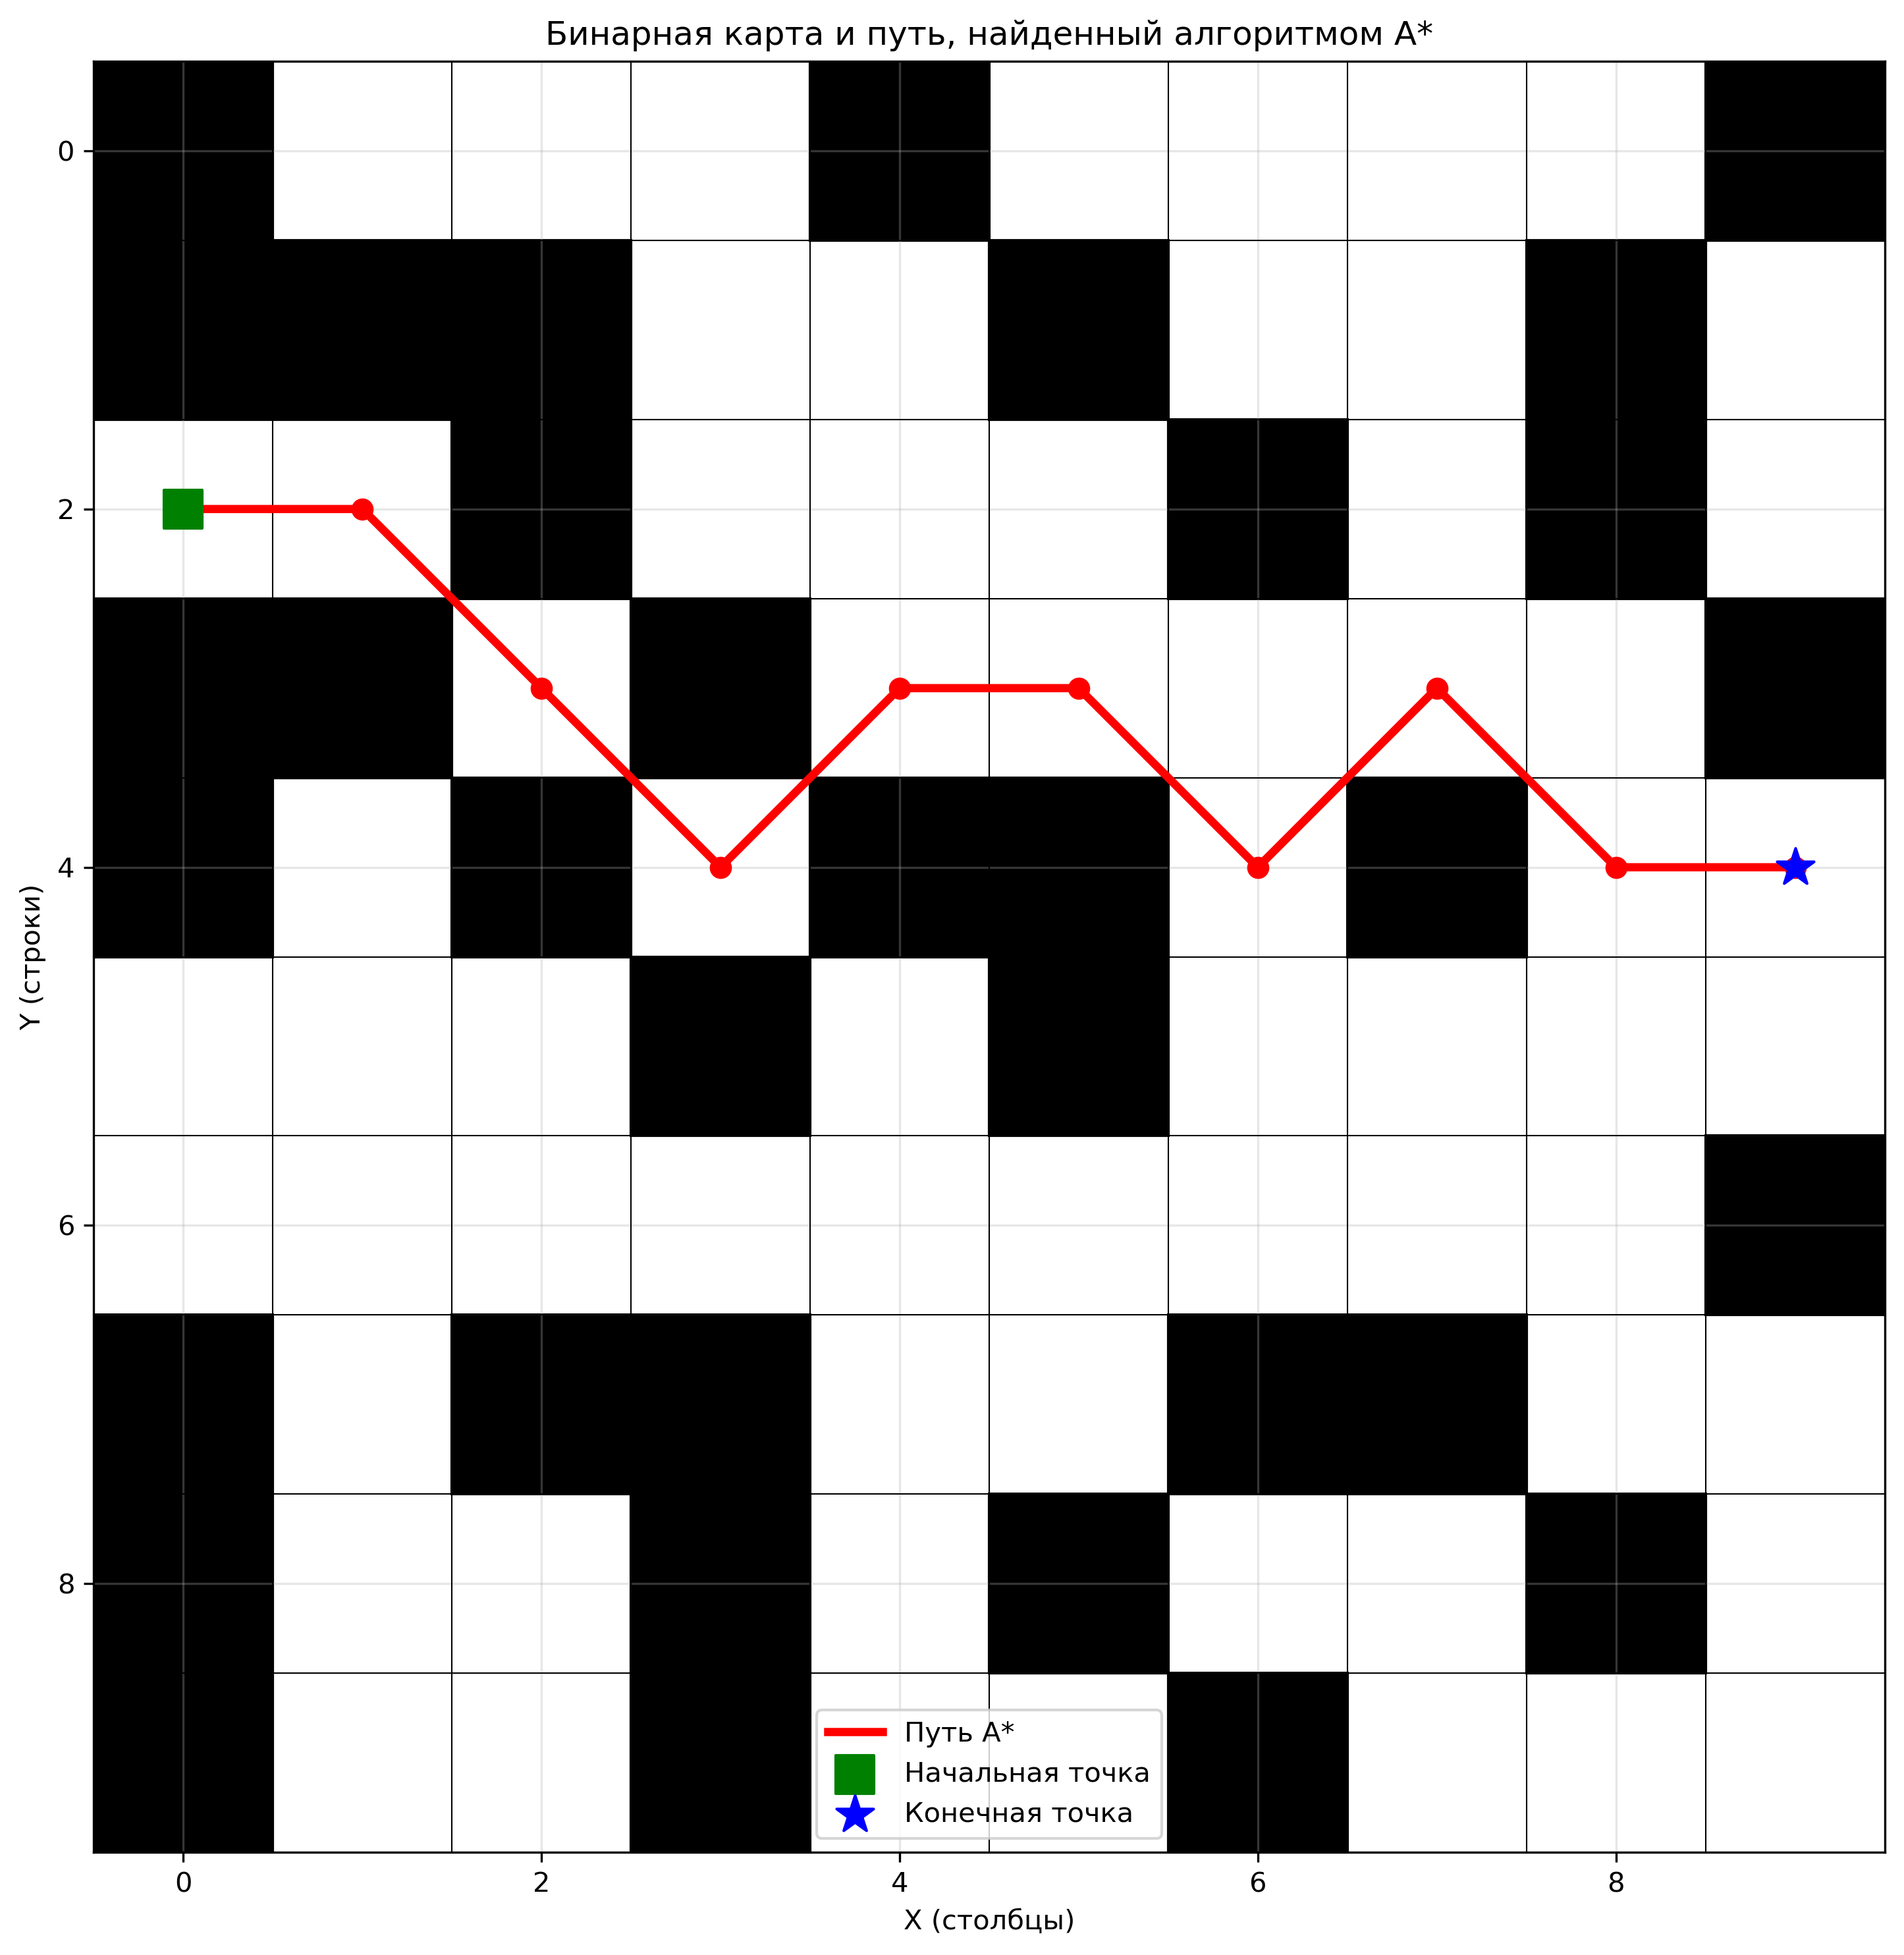
\includegraphics[width=0.8\textwidth]{task1/astar_path.png}
\caption{Бинарная карта и путь, найденный алгоритмом A*}
\label{fig:astar_path}
\end{figure}

Параметры найденного пути:
\begin{itemize}
\item Длина пути: 10 ячеек
\item Количество поворотов: 7
\item Начальная точка: (2, 0)
\item Конечная точка: (4, 9)
\end{itemize}

\subsection{Сравнение траекторий с разной гладкостью}

На рисунке \ref{fig:trajectories_comparison} представлено сравнение всех сгенерированных траекторий.

\begin{figure}[H]
\centering
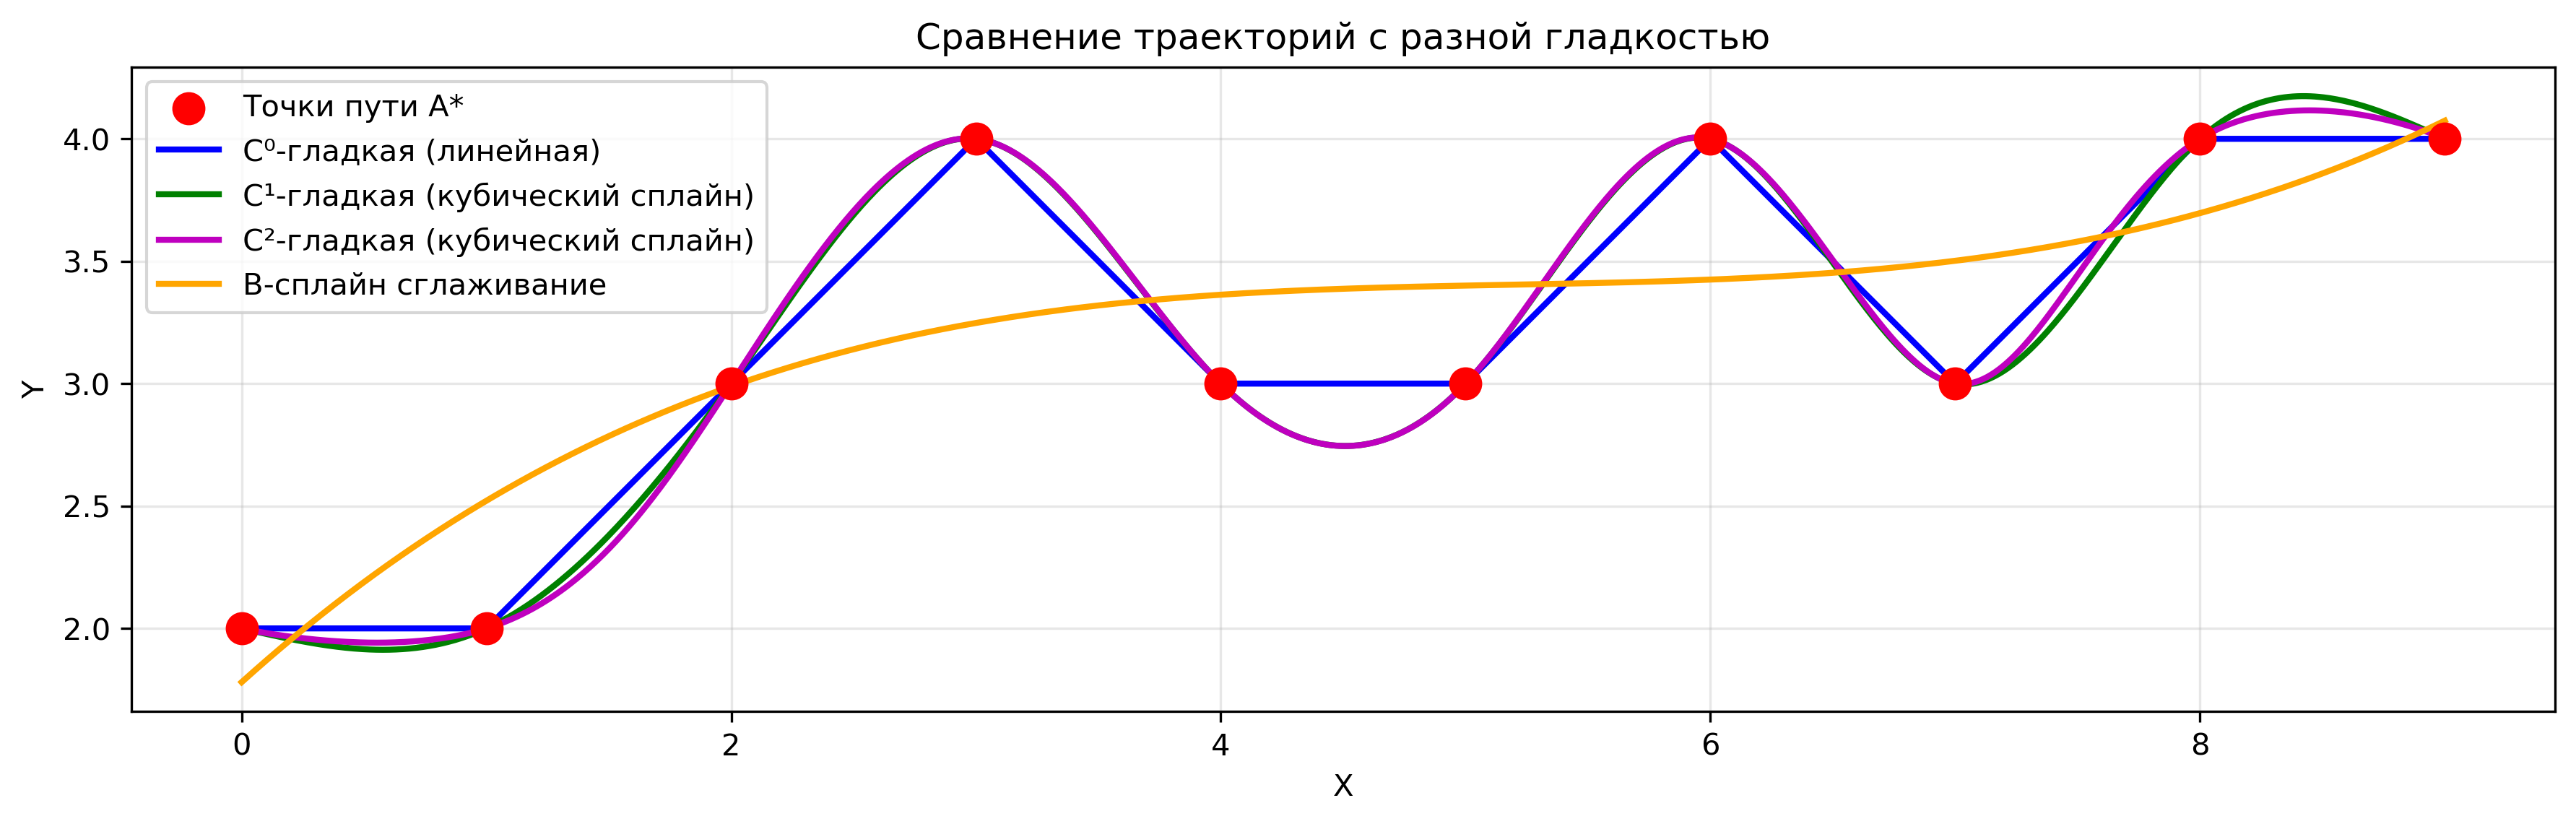
\includegraphics[width=0.9\textwidth]{task2/trajectories_comparison.png}
\caption{Сравнение траекторий с разной гладкостью}
\label{fig:trajectories_comparison}
\end{figure}

\subsection{Анализ кривизн траекторий}

На рисунке \ref{fig:curvature_comparison} представлено сравнение кривизн всех траекторий.

\begin{figure}[H]
\centering
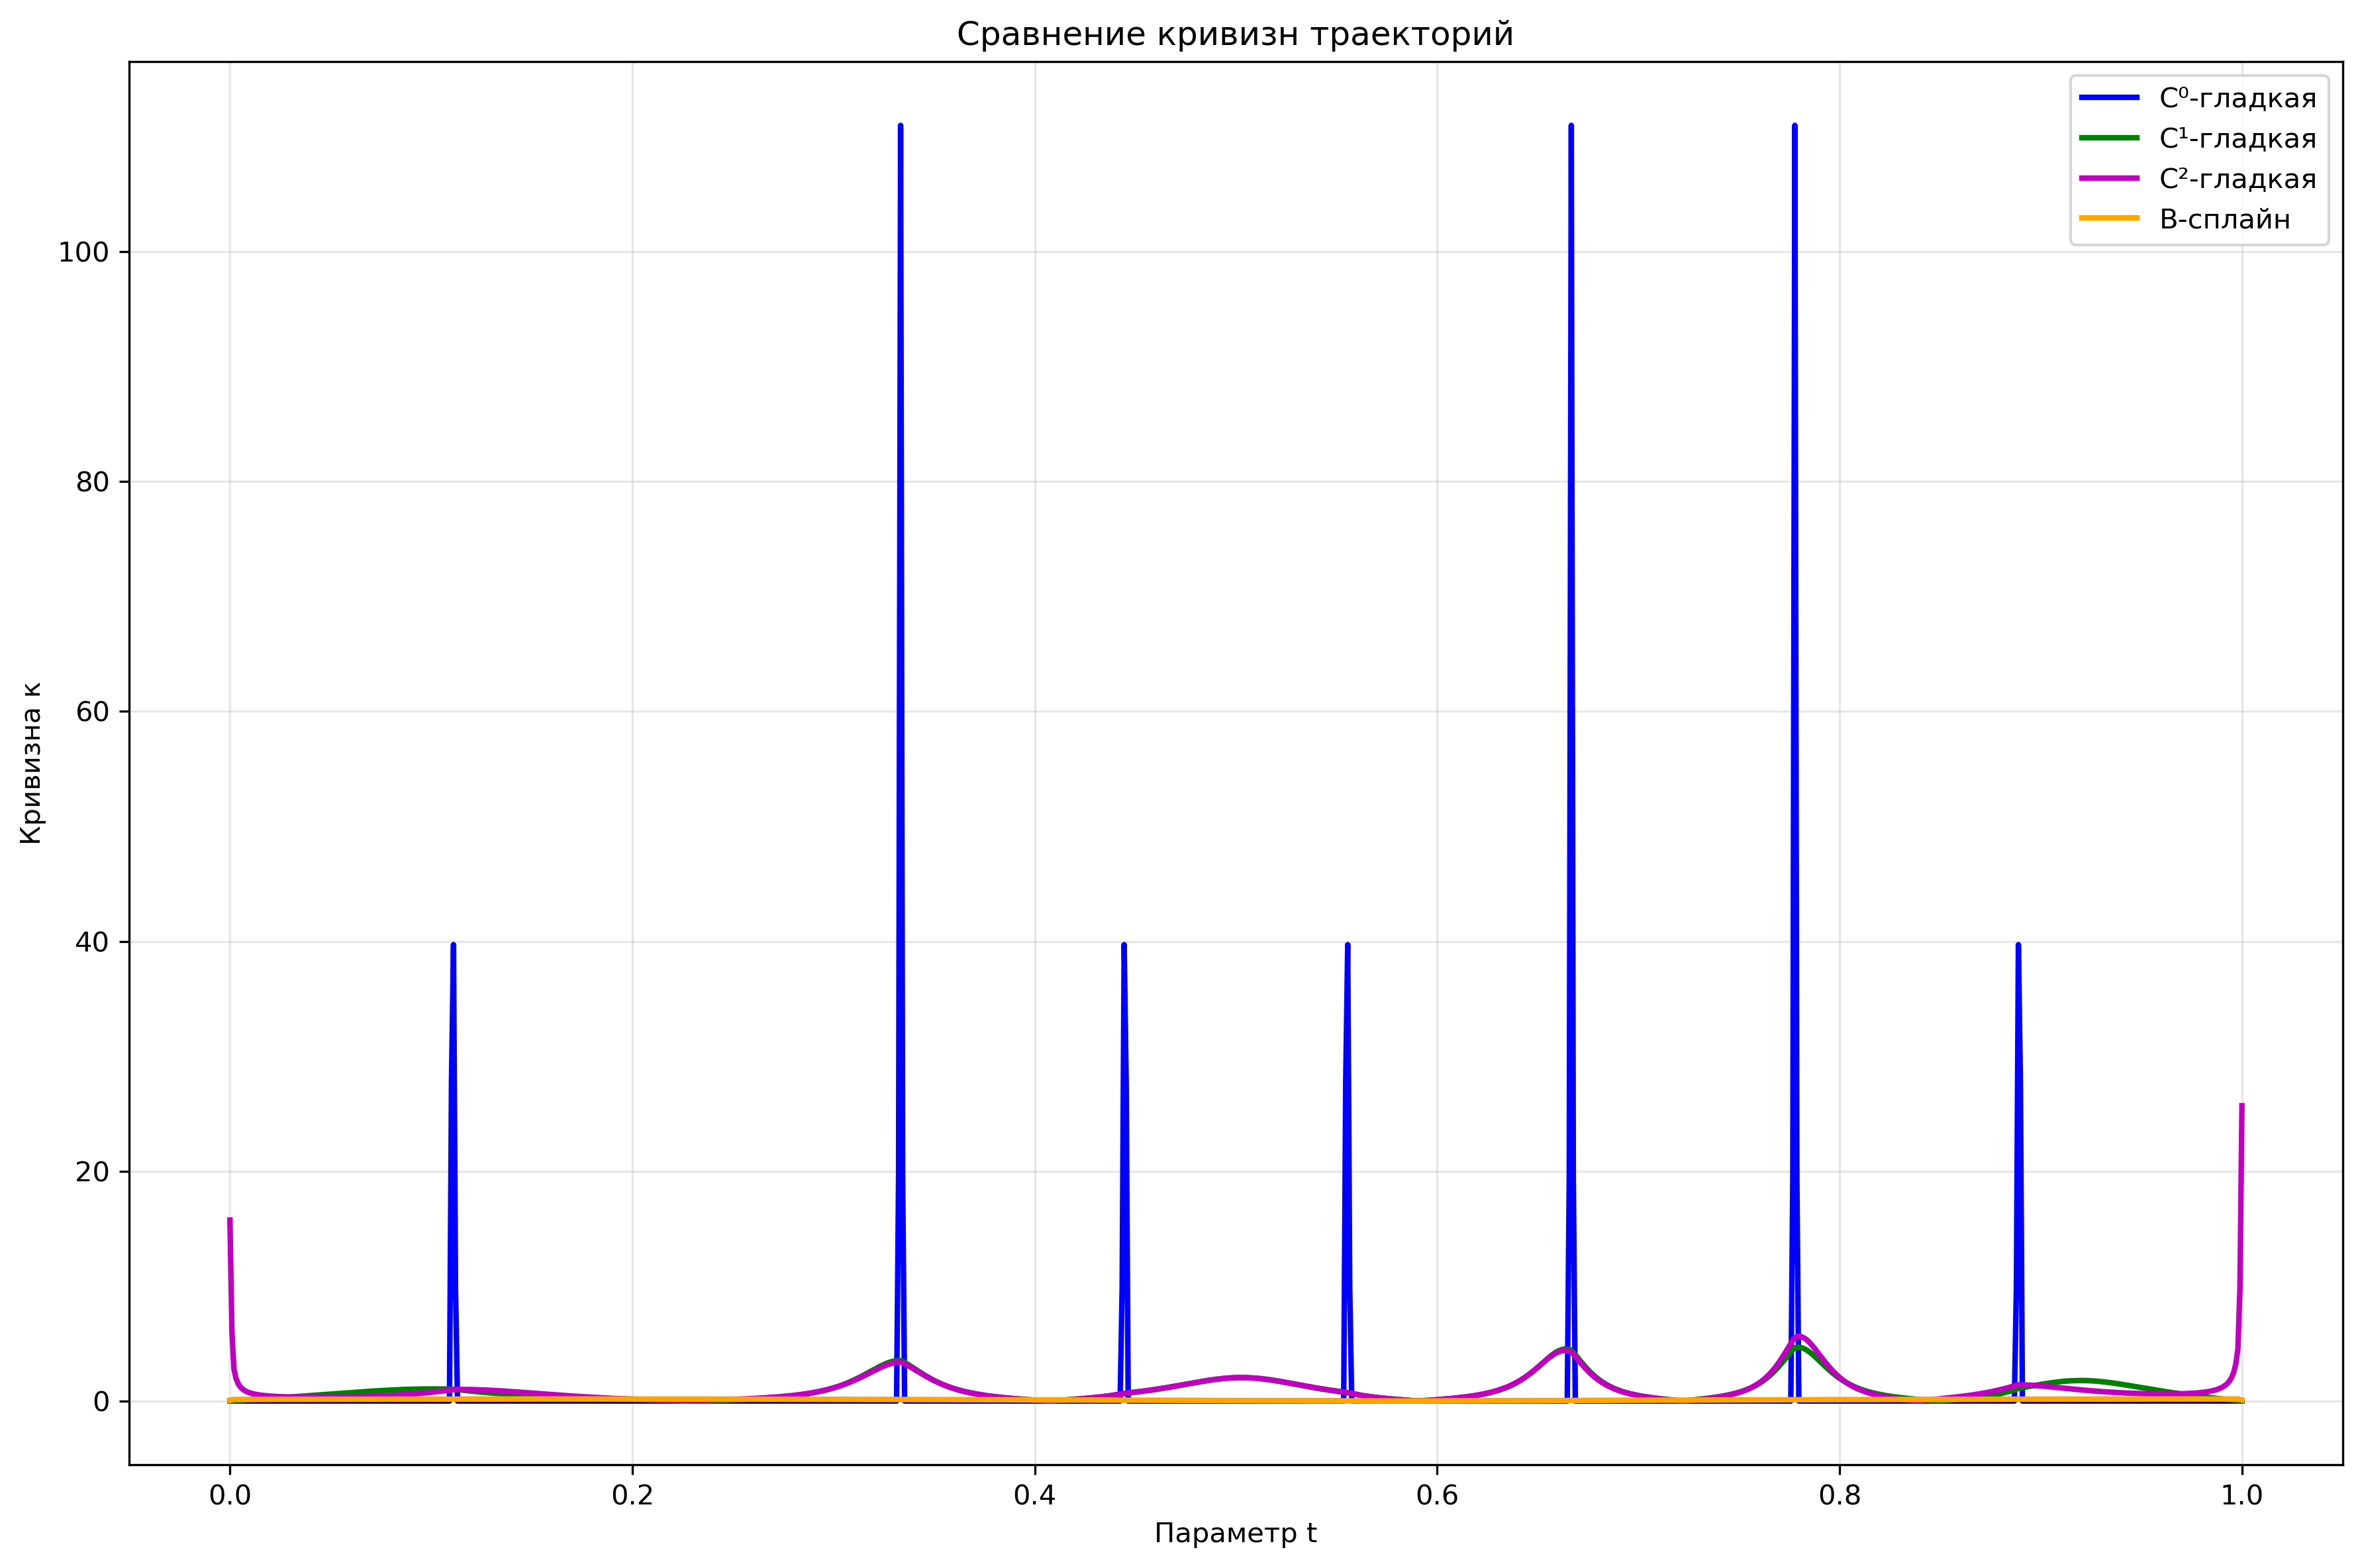
\includegraphics[width=0.9\textwidth]{task2/curvature_comparison.png}
\caption{Сравнение кривизн траекторий}
\label{fig:curvature_comparison}
\end{figure}

Статистика кривизн:
\begin{itemize}
\item C$^0$-гладкая: средняя = 0.7598, максимальная = 111.0000
\item C$^1$-гладкая: средняя = 0.9710, максимальная = 4.6861
\item C$^2$-гладкая: средняя = 1.0420, максимальная = 25.6972
\item B-сплайн: средняя = 0.1189, максимальная = 0.1800
\end{itemize}

\section{Выводы}

\begin{enumerate}
\item Алгоритм A* успешно нашел путь длиной 10 ячеек с 7 поворотами, что удовлетворяет требованиям задания.

\item C$^0$-гладкая траектория имеет наибольшую максимальную кривизну (111.0) из-за резких углов в точках поворота, что делает её непригодной для практического использования.

\item C$^1$-гладкая траектория показывает значительное улучшение по сравнению с C$^0$-гладкой, максимальная кривизна снизилась до 4.69.

\item C$^2$-гладкая траектория имеет промежуточные характеристики между C$^1$-гладкой и B-сплайном.

\item B-сплайн сглаживание обеспечивает наилучшие характеристики с точки зрения гладкости: минимальная средняя кривизна (0.119) и максимальная кривизна (0.18), что делает эту траекторию наиболее подходящей для практического применения.

\item Все траектории с гладкостью выше C$^0$ показывают значительное улучшение характеристик по сравнению с кусочно-линейной траекторией.
\end{enumerate}

                                     % Введение
% \input{3_chap1}                                     % Первая глава
% \input{4_chap2}                                     % Вторая глава
% \input{5_chap3}                                     % Третья глава

\printbibliography[title=Список использованных источников] % Автособираемый список литературы

\end{document}